% \input{\pathsections "sec bohr-wheeler"}

\section{Liquid Drop Model: Non--Spherical}

\begin{frame}\frametitle{Comparison of Liquid Drop Models}
\begin{table}[htp]
%\caption{default}
\begin{center}
\begin{tabular}{cc}
	Constant Radius & Variable Radius \\\hline
	\ \\
	\includegraphics[ width= 2in ]{\pLocalGraphics liquid-drop-sphere} & 
	\includegraphics[ width= 2in ]{\pLocalGraphics liquid-drop-balls} 
\end{tabular}
\end{center}
%\label{default}
\end{table}%
\end{frame}
%
\begin{frame}\frametitle{Historical Survey}
\center
	\href{\reedBook}{
	\begin{overpic}[ scale = 0.105 ]
	{\pLocalGraphics Manhattan}
	\end{overpic}}
\center
\footnotesize{
Appendix E: Formal Derivation of the \bl{Bohr–Wheeler Spontaneous Fission Limit}.} 
\end{frame}
%
\begin{frame}\frametitle{Summary of Liquid Drop Model\jumpLittle}
\begin{enumerate}
	\item Nucleus is liquid drop of \bl{variable radius}
	\item Fluid is incompressible
	\item Volume is conserved
\end{enumerate}
\end{frame}


%%%   %%%   %%%   %%%
\subsection{The Mechanism of Nuclear Fission}
\begin{frame}\frametitle{1939 Paper on \href{https://en.wikipedia.org/wiki/Nuclear\_fission}{Nuclear Fission}}
\center
	\href{\bohrPaper}{
	\begin{overpic}[ scale = 0.8]
	{\pLocalGraphics paper-bohr-wheeler-a}
		%\put(24,43){$Z=92$}
	\put(85.5,28) {\includegraphics[ width = 1cm ]{\pLocalGraphics medal}}
	\end{overpic}}
\end{frame}


\begin{frame}\frametitle{Deformations from Sphericity}
\center
	\href{\bohrPaper}{\begin{overpic}[ scale = 0.9]
	{\pLocalGraphics bw-01a}
	\end{overpic}}
\end{frame}

\begin{frame}\frametitle{Bohr-Wheeler Derivation}
\center
	\href{\bohrPaper}{\begin{overpic}[ scale = 0.75]
	{\pLocalGraphics bw-formula-a}
	\end{overpic}}
\end{frame}

\begin{frame}\frametitle{Express Radius as a Function of Polar Angle}
%
\begin{equation}
	\mg{\xcancel{\bk{r = R_{0}}}}
%\label{eq:name}
\end{equation}
$$ \Downarrow $$
\begin{equation}
	r(\theta) = R_{0}\paren{\bwexpa}
\label{eq:bw-radius}
\end{equation}
\end{frame}

\begin{frame}\frametitle{Express Radius as a Function of Polar Angle\jumpLittle}
%
Adjust $ \azero$, $ \atwo$ so that \rd{volume is conserved}:
\begin{equation}
	r(\theta) = R_{0}\paren{\bwexpa}
\tag{\ref{eq:bw-radius}}
\end{equation}
\end{frame}

%%%   %%%   %%%   %%%
\subsection{Legendre Polynomials}
\begin{frame}\frametitle{Why Legendre Polynomials?}
	Problem: \rd{Planetary Orbits}\\[10pt]
	\bl{Recherches sur la figure des plan\`etes}\\[10pt]
\href{Adrien-Marie Legendre}{AM Legendre}\\
Mémoires de l'Acad\'emie Royale des sciences, 1784
\end{frame}

\begin{frame}\frametitle{Why Legendre Polynomials?}
\center
	\href{https://www.coursehero.com/study-guides/astronomy/orbits-in-the-solar-system/}{
	\begin{overpic}[ scale = 0.25 ]
	{\pLocalGraphics orbits}
		%\put(0,0){Text}
	\end{overpic}}
\end{frame}

\begin{frame}\frametitle{Why Legendre Polynomials?}
\center
	\href{https://www.coursehero.com/study-guides/astronomy/orbits-in-the-solar-system/}{
	\begin{overpic}[ scale = 0.25 ]
	{\pLocalGraphics orbits}
		\put(100,70){\href{https://bogan.ca/orbits/ellipse.html}{Orbit types:}}
		\put(100,62){Circular}
		\put(100,54){Elliptical}
		\put(100,46){Parabolic}
		\put(100,38){Hyperbolic}
	\end{overpic}}
\end{frame}

\begin{frame}\frametitle{\href{https://en.wikipedia.org/wiki/Legendre\_polynomials\#Expanding\_a\_1/r\_potential}{Expansion} of the \href{https://en.wikipedia.org/wiki/Newtonian\_potential}{Newtonian Potential}}
\begin{equation}
%	\frac{1}{x-x'} = \frac{1}{\sqrt{r^{2}+r'^{2} -2rr' \cos \gamma}} = \sum_{k=0}^{\infty}\frac{r'^{k}}{r^{k+1}} \bl{P_{k}}\paren{\cos \gamma}
	\frac{1}{\normt{d}} = \frac{1}{\sqrt{R^{2}+r^{2} -2Rr \cos \gamma}} = \sum_{k=0}^{\infty}\frac{r^{k}}{R^{k+1}} \bl{P_{k}}\paren{\cos \gamma}
\end{equation}
\end{frame}

\begin{frame}\frametitle{\href{https://en.wikipedia.org/wiki/Legendre\_polynomials\#Expanding\_a\_1/r\_potential}{Expansion} of the \href{https://en.wikipedia.org/wiki/Newtonian\_potential}{Newtonian Potential}}
\begin{equation}
%	\frac{1}{x-x'} = \frac{1}{\sqrt{r^{2}+r'^{2} -2rr' \cos \gamma}} = \sum_{k=0}^{\infty}\frac{r'^{k}}{r^{k+1}} \bl{P_{k}}\paren{\cos \gamma}
	\frac{1}{\normt{d}} = \frac{1}{\sqrt{R^{2}+r^{2} -2Rr \cos \gamma}} = \sum_{k=0}^{\infty}\frac{r^{k}}{R^{k+1}} \bl{P_{k}}\paren{\cos \gamma}
\end{equation}
$$\Uparrow$$
\center
I am the Law of Cosines
\end{frame}

\begin{frame}\frametitle{\LawOfCosinesWikipedia}
\center
	%\href{}{
	\begin{overpic}[ scale = 0.8 ]
		{\pLocalGraphics law-of-cosines}
		\put(14, 25)	{\colorbox{white}{$\rd{R}$}}
		\put(42, 39)	{\colorbox{white}{$\rd{r}$}}
		\put(30, 15)	{\colorbox{white}{$\bl{d}$}}
	\end{overpic}
\end{frame}

\begin{frame}\frametitle{\href{https://en.wikipedia.org/wiki/Legendre\_polynomials\#Expanding\_a\_1/r\_potential}{Expansion} of the \href{https://en.wikipedia.org/wiki/Newtonian\_potential}{Newtonian Potential}}
\begin{equation}
%	\frac{1}{x-x'} = \frac{1}{\sqrt{r^{2}+r'^{2} -2rr' \cos \gamma}} = \sum_{k=0}^{\infty}\frac{r'^{k}}{r^{k+1}} \bl{P_{k}}\paren{\cos \gamma}
	\frac{1}{\normt{\color{blue}{d}}} = \frac{1}{\sqrt{\rd{R^{2}}+ \rd{r^{2}} -\rd{2Rr \cos \gamma}}} = \sum_{k=0}^{\infty}\frac{r^{k}}{R^{k+1}} \bl{P_{k}}\paren{\cos \gamma}
\end{equation}
$$\Uparrow$$
\center
I am the Law of Cosines
\end{frame}

\begin{frame}\frametitle{\href{https://en.wikipedia.org/wiki/Effective_potential}{Effective Potential}}
\center
\input{\pSections "fig-effective-potential"}
\end{frame}

\begin{frame}\frametitle{\href{https://en.wikipedia.org/wiki/Effective_potential}{Effective Potential}}
\center
\input{\pSections "fig-effective-potential-a"}
\end{frame}


%\begin{tikzpicture}
%% Set horizontal range 
%\pgfmathsetmacro{\nx}{8}
%% Set vertical range 
%\pgfmathsetmacro{\ny}{2.5}
%
%\pgfmathsetmacro{\xmin}{2*(sqrt(\ny+1)-1)/\ny}
%\pgfmathsetmacro{\xmint}{2/sqrt(\ny)}
%\pgfmathsetmacro{\xminb}{4/\ny}
%\pgfmathsetmacro{\xmax}{2*\nx}
%
%\begin{axis}[xmin=0,xmax=\xmax,axis x line*=middle, axis y line*=left, xtick=\empty, ytick=\empty]
%    \addplot[red,thick,domain=\xmin:\xmax,samples=100]{1/x^2-1/x};
%    \addplot[domain=\xminb:\xmax,samples=100]{-1/x};
%    \addplot[domain=\xmint:\xmax,samples=100]{1/x^2};
%\end{axis}
%\end{tikzpicture}
%
%
\begin{frame}\frametitle{Deformations from Sphericity}
\begin{table}[htp]
%\caption{default}
\begin{center}
	\begin{tabular}{ll}
		 %
	\qquad even parity & \qquad odd parity \\
		 %
	\includegraphics[ width = 3.5cm ]{\pLocalGraphics legendre-even} &
	\includegraphics[ width = 3.5cm ]{\pLocalGraphics legendre-odd} \\
		 %
		
	\small{$P_{0}(x) = 1$} & 
	\small{$P_{1}(x) = x$} \\
	\small{$P_{2}(x) = \pr{\frac{1}{2}\paren{3x^{2} - 1}}$} & 
	\small{$P_{3}(x) = \frac{1}{2}\paren{5x^{3} - 3x}$} \\
	\small{$P_{4}(x) = \frac{1}{8}\paren{35x^{4} - 30x^{2} + 3}$} & 
	\small{$P_{5}(x) = \frac{1}{8}\paren{63x^{5} - 70x^{3} + 15x}$} \\
		 %
	\end{tabular}
\end{center}
%\label{tab:label}
\end{table}%
\end{frame}

\begin{frame}\frametitle{Mathematical Properties of \legendremathworld}
\begin{enumerate}
	\item Norm: $\displaystyle\int_{-1}^{1}\bl{P_{j}(x)P_{k}(x)}dx = \frac{1}{2k+1}\delta_{j}^{k}$
	\item \href{https://mathworld.wolfram.com/LegendreDifferentialEquation.html}{Solution} to $(1-x^{2}) \bl{P_{n}(x)}'' -2x \bl{P_{n}(x)}' + n(n+1)\bl{P_{n}(x)} = 0$\\[10pt]
	\item \href{https://en.wikipedia.org/wiki/Sturm\%E2\%80\%93Liouville_theory}{Sturm--Liouville} Form: $\frac{d}{dx}\paren{\paren{1-x^{2}}\frac{d}{dx}}\bl{P(x)} = - \lambda \bl{P(x)}$\\[10pt]
	\item \href{https://en.wikipedia.org/wiki/Rodrigues\%27\_formula}{Rodrigues' formula}: $\bl{P_{n}(x)} = \frac{1}{2^{n}n!}\frac{d^{n}}{dx^{n}}\paren{x^{2} - 1}^{n} $\\[10pt]
	\item \href{https://mathworld.wolfram.com/OrthogonalDecomposition.html}{Decomposition}: $f_{n}(x) = \displaystyle \sum_{k=0}^{l}a_{k} \bl{P_{k}(x)}$, $a_{k} = \displaystyle\frac{2k+1}{2}\int_{-1}^{1} f(x) \bl{P_{k}(x)}$\\[10pt]
	\item \href{https://mathworld.wolfram.com/CompleteOrthogonalSystem.html}{Completeness}: $\displaystyle\sum_{k=0}^{\infty}\frac{2k+1}{2}\bl{P_{k}(x)P_{k}(y)} = \delta(x-y)$, $x,y\in\brac{-1,1}$
\end{enumerate}
\end{frame}

\begin{frame}\frametitle{Mathematical Properties of \legendremathworld\jumpLittle}
\begin{enumerate}
	\item First Use: $\legendreFirst$
	\item Generating function: $\legendreGenerate{}$
	\item \href{https://mathworld.wolfram.com/MonicPolynomial.html}{Monic} \href{https://mathworld.wolfram.com/Gram-SchmidtOrthonormalization.html}{Gram-Schmidt} on $(1, x, x^{2}, x^{3}, \dots)$ over $x\in\brac{-1,1}$
	\item \href{https://en.wikipedia.org/wiki/Legendre\_polynomials\#Definition\_via\_generating\_function}{Bonnet’s} Recursion Formula: $\legendreBonnet$
	\item a.k.a. \href{https://mathworld.wolfram.com/LegendrePolynomial.html}{Legendre functions of the first kind}
	\item a.k.a. \href{https://mathworld.wolfram.com/ZonalHarmonic.html}{zonal harmonics}
\end{enumerate}
\end{frame}

%%%   %%%   %%%   %%%
\subsection{Integration in Spherical Coordinates}
%\begin{frame}\frametitle{\href{https://tex.stackexchange.com/questions/159445/draw-in-cylindrical-and-spherical-coordinates/159452}{Volume Element $dV$ in Spherical Coordinates}}
%	\center
%	\footnotesize{
%%	\href{https://tex.stackexchange.com/questions/159445/draw-in-cylindrical-and-spherical-coordinates/159452}{\input{\pSections "fig-differential-volume"}}}
%	\input{\pSections "fig-differential-volume"}}
%\end{frame}
\begin{frame}\frametitle{How To Compute Volume of Deformed Nucleus?}
\begin{table}[htp]
%\caption{default}
\begin{center}
\begin{tabular}{cc}
	$V = \tfrac{4}{3}\pi R_{0}^{3}$ & $V = \,???$ \\
	\ \\
	\includegraphics[ width= 2in ]{\pLocalGraphics liquid-drop-sphere} & 
	\includegraphics[ width= 2in ]{\pLocalGraphics liquid-drop-balls} 
\end{tabular}
\end{center}
%\label{default}
\end{table}
\end{frame}

\begin{frame}\frametitle{\href{https://tex.stackexchange.com/questions/159445/draw-in-cylindrical-and-spherical-coordinates/159452}{Draw Spherical Volume Element}}
	\footnotesize{
%	\href{https://tex.stackexchange.com/questions/159445/draw-in-cylindrical-and-spherical-coordinates/159452}{\input{\pSections "fig-differential-volume"}}}
	\input{\pSections "fig-differential-volume"}}
\end{frame}

\begin{frame}\frametitle{\href{https://tex.stackexchange.com/questions/159445/draw-in-cylindrical-and-spherical-coordinates/159452}{Define Angular Range}}
	\footnotesize{
	\input{\pSections "fig-differential-volume"}
	\begin{textblock}{4}(11,7)
		$\theta \in \brac{0, \pi}$ 
	\end{textblock}
	\begin{textblock}{4}(11,8)
		$\phi  \in \brac{0, 2\pi}$ 
	\end{textblock}}
\end{frame}

\begin{frame}\frametitle{\href{https://tex.stackexchange.com/questions/159445/draw-in-cylindrical-and-spherical-coordinates/159452}{Spherical Volume Element \color{yellow}{$dV = \dV$}}}
	\footnotesize{
	\input{\pSections "fig-differential-volume"}
	\begin{textblock}{4}(11,7)
		$\theta \in \brac{0, \pi}$ 
	\end{textblock}
	\begin{textblock}{4}(11,8)
		$\phi  \in \brac{0, 2\pi}$ 
	\end{textblock}
	\begin{textblock}{7}(10,9.5)
		$dV = \vElement$ 
	\end{textblock}}
\end{frame}

\begin{frame}\frametitle{\href{https://tex.stackexchange.com/questions/159445/draw-in-cylindrical-and-spherical-coordinates/159452}{Volume Integral \color{yellow}{$V = \iiint dV$}}}
	\footnotesize{
	\input{\pSections "fig-differential-volume"}
	\begin{textblock}{4}(11,7)
		\mg{$\theta \in \brac{0, \pi}$} 
	\end{textblock}
	\begin{textblock}{4}(11,8)
		\mg{$\phi  \in \brac{0, 2\pi}$ }
	\end{textblock}
	\begin{textblock}{7}(10,9.5)
		$dV = \vElement$ 
	\end{textblock}
	\begin{textblock}{10}(9.25,11.5)
		$V = \iiint dV$ 
	\end{textblock}
	\begin{textblock}{10}(9.7,12.5)
		$=  \displaystyle\vIntE$ 
	\end{textblock}}
\end{frame}

%\begin{frame}\frametitle{\href{https://tex.stackexchange.com/questions/159445/draw-in-cylindrical-and-spherical-coordinates/159452}{Spherical Volume Element \color{yellow}{$dV = \dV$}}}
%\begin{columns}[T]%beamer
%\column{0.5\textwidth}
%%	\href{https://tex.stackexchange.com/questions/159445/draw-in-cylindrical-and-spherical-coordinates/159452}{\input{\pSections "fig-differential-volume"}}}
%	\input{\pSections "fig-differential-volume"}
%\end{columns}
%	\footnotesize{
%	\begin{textblock}{4}(2,7)
%		\mg{$0 \le \theta \le \pi$} 
%	\end{textblock}
%	\begin{textblock}{4}(2,8)
%		\mg{$0 \le \phi \le 2\pi$} 
%	\end{textblock}
%	\begin{textblock}{7}(1,9)
%		\mg{$dV = \vElement$} 
%	\end{textblock}
%	\pause
%	\begin{textblock}{9}(0.5,10.3)
%		$V = \iiint dV= \displaystyle\vIntB$ 
%	\end{textblock}}
%%	\begin{textblock}{9}(0.85,9.5)
%%		$V = \iiint dV$ 
%%	\end{textblock}
%%	\begin{textblock}{9}(1.2,10.3)
%%		$= \displaystyle\vIntB$ 
%%	\end{textblock}}
%\end{frame}
%
%\begin{frame}\frametitle{\href{https://tex.stackexchange.com/questions/159445/draw-in-cylindrical-and-spherical-coordinates/159452}{Spherical Volume Element \color{yellow}{$dV = \dV$}}}
%	\footnotesize{
%%	\href{https://tex.stackexchange.com/questions/159445/draw-in-cylindrical-and-spherical-coordinates/159452}{\input{\pSections "fig-differential-volume"}}}
%	\input{\pSections "fig-differential-volume"}}
%	\begin{textblock}{4}(11,7)
%		\mg{$0 \le \theta \le \pi$} 
%	\end{textblock}
%	\begin{textblock}{4}(11,8)
%		\mg{$0 \le \phi \le 2\pi$} 
%	\end{textblock}
%	\begin{textblock}{7}(10,10)
%		\mg{$dV = \vElement$} 
%	\end{textblock}
%	\pause
%	\begin{textblock}{9}(7,5)
%		$V = \iiint dV = \vIntA$ 
%	\end{textblock}
%\end{frame}
%
%\begin{frame}\frametitle{\href{https://tex.stackexchange.com/questions/159445/draw-in-cylindrical-and-spherical-coordinates/159452}{Spherical Volume Element $dV = \dV$}}
%	\center
%	\footnotesize{
%%	\href{https://tex.stackexchange.com/questions/159445/draw-in-cylindrical-and-spherical-coordinates/159452}{\input{\pSections "fig-differential-volume"}}}
%	\input{\pSections "fig-differential-volume"}}
%	\begin{textblock}{4}(0,5)
%		$0 \le \theta \le \pi$ 
%	\end{textblock}
%	\begin{textblock}{4}(0,4)
%		$0 \le \phi \le 2\pi$ 
%	\end{textblock}
%	\begin{textblock}{7}(3,7)
%		$dV = dr \paren{r d\phi} \paren{r\sin{\theta}d\theta}$ 
%	\end{textblock}
%\end{frame}
%\begin{frame}\frametitle{Deformations from Sphericity}
%Vary the radius, keep volume fixed:
%%
%\begin{equation}
%	dV = \vElement
%%\label{eq:name}
%\end{equation}
%%
%\begin{equation}
%	V = \int \int \int dV = \displaystyle\vIntC
%%\label{eq:name}
%\end{equation}
%\end{frame}

\begin{frame}\frametitle{Deformations from Sphericity}
Constant radius, spherical volume:
%
\begin{equation}
	dV = \vElement
%\label{eq:name}
\end{equation}
%
\begin{equation}
	V = \iiint dV = \displaystyle\vIntE = \sphereVolume
%\label{eq:name}
\end{equation}
\pause
Vary the radius, keep volume fixed:
\begin{equation}
	V(\theta) = \int_{\theta=0}^{\pi} \int_{\rho = 0}^{r(\theta)} \int_{\phi=0}^{2\pi} \rho^{2} \sin{\theta}\, d\theta\, d\rho\, d\phi
%\label{eq:name}
\end{equation}
%$$\vIntA$$
\end{frame}

%\begin{frame}\frametitle{Deformations from Sphericity}
%Vary the radius, keep volume fixed:
%%
%\begin{equation}
%	dV = \vElement
%%\label{eq:name}
%\end{equation}
%%
%\begin{equation}
%	V = \int \int \int dV = \displaystyle\vIntC
%%\label{eq:name}
%\end{equation}
%\pause
%Fubini theorem:
%\begin{equation}
%	V(\theta) = \int_{\theta=0}^{\pi} \int_{\rho = 0}^{r(\theta)} \int_{\phi=0}^{2\pi} \rho^{2} \sin{\theta}\, d\theta\, d\rho\, d\phi
%%\label{eq:name}
%\end{equation}
%$$\vIntA$$
%\end{frame}

\begin{frame}\frametitle{Can We Switch The Order of Integration?}
\begin{equation}
	\displaystyle\vIntE \,
		\rd{\overset{?}{=}} 
			\int\limits_{\theta=0}^{\pi} \int\limits_{\rho = 0}^{r(\theta)} \int\limits_{\phi=0}^{2\pi} \rho^{2} \sin{\theta}\, d\theta\, \bl{d\rho}\, \rd{d\phi}
%\label{eq:name}
\end{equation}
\end{frame}

%\begin{frame}\frametitle{Can We Switch The Order of Integration?}
%\begin{equation}
%	\int_{\theta=0}^{\pi} \int_{\rho = 0}^{r(\theta)} \int_{\phi=0}^{2\pi} dr \paren{\rho d\phi} \paren{r\sin{\theta}d\theta} \rd{\overset{?}{=}} \int_{\theta=0}^{\pi} \int_{\rho = 0}^{r(\theta)} \int_{\phi=0}^{2\pi} \rho^{2} \sin{\theta}\, d\theta\, d\rho\, d\phi
%%\label{eq:name}
%\end{equation}
%\end{frame}
%
\begin{frame}\frametitle{\color{yellow}{Yes}, We Can Switch The Order of Integration}
The \href{https://mathworld.wolfram.com/FubiniTheorem.html}{Fubini Theorem} relates \bl{multiple integrals} to \bl{iterated integrals}:
\input{\pSections thm-fubini}
\end{frame}

\begin{frame}\frametitle{First Volume Integral: $\phi$ integration}
\begin{equation}
	\begin{array}{rcl}
	V(\theta) &=& \displaystyle\int_{\theta=0}^{\pi} \int_{\rho = 0}^{r(\theta)} \bl{\int_{\phi=0}^{2\pi}} \rho^{2} \sin{\theta}\,  d\theta\, d\rho\,  \bl{d\phi} \\[18pt]
		&=& \displaystyle\int_{\theta=0}^{\pi} \int_{\rho = 0}^{r(\theta)} \rho^{2} \sin{\theta}\,  d\theta \times \bl{\phi} \bl{\eval_{0}^{2\pi}} \\[18pt]
		&=& \bl{2\pi} \displaystyle\int_{\theta=0}^{\pi} \int_{\rho = 0}^{r(\theta)} \rho^{2} \sin{\theta}\,  d\theta\,  d\rho \\
	\end{array}
\end{equation}
\end{frame}

\begin{frame}\frametitle{Second Volume Integral: $\rho$ integration}
\begin{equation}
	\begin{array}{rcl}
	V(\theta) &=& 2\pi \displaystyle \int_{\theta=0}^{\pi} \bl{\int_{\rho = 0}^{r(\theta)}}  \bl{\rho^{2}} \sin{\theta} \, d\theta\,  \bl{d\rho} \\[15pt]
	\pause
		&=& \frac{2\pi}{3} \displaystyle \int_{\theta=0}^{\pi} \bl{\rho^{3}} \sin{\theta} \,d\theta \, \bl{\eval_{0}^{r(\theta)}}  \\[15pt]
	\pause
		&=& \frac{2\pi}{3} \displaystyle \int_{\theta=0}^{\pi} \bl{r^{3}(\theta)}\sin{\theta} \,d\theta   \\[15pt]
	\pause
		&=& \frac{2\pi}{3} \displaystyle \int_{\theta=0}^{\pi} \paren{R_{0}\paren{\bwexpa}}^{3} \sin{\theta} \, d\theta \\
	\end{array}
\end{equation}
\end{frame}

\begin{frame}\frametitle{Radial Variations Must Conserve Volume}
%\begin{equation}
%	\frac{4\pi}{3} R_{0}^{3} =  \frac{2\pi}{3} \displaystyle \int_{\theta=0}^{\pi} r^{3}(\theta) \sin{\theta} \, d\theta
%\end{equation}
%
Using equation \ref{eq:bw-radius} for the Legendre expansion...
\begin{equation}
	\begin{array}{rcl}
		\frac{4\pi}{3} R_{0}^{3} &=&  \frac{2\pi}{3} \displaystyle \int_{\theta=0}^{\pi} r^{3}(\theta) \sin{\theta} \, d\theta \\[10pt]
		%&=& \frac{2\pi}{3} \displaystyle \int_{\theta=0}^{\pi} \paren{R_{0}\paren{\bwexpa}}^{3} \sin{\theta} \, d\theta \\[10pt]
		&=& \frac{2\pi}{3} R_{0}^{3} \displaystyle \int_{\theta=0}^{\pi} \paren{\bwexpa}^{3} \sin{\theta} \, d\theta \\
	\end{array}
%\label{eq:name}
\end{equation}
Conclusion: To \rd{conserve volume}, 
\begin{equation}
	%\begin{split}
	1 = \int_{\theta=0}^{\pi} \paren{\bwexpa}^{3} \sin{\theta} \, d\theta
	%\end{split}
\label{eq:conserve}
\end{equation}
\end{frame}

\begin{frame}\frametitle{Express Legendre Polynomials as Monomials\jumpLittle}
$$\mg{\int_{\theta=0}^{\pi}} \paren{\bwexpa}^{3}  \mg{\sin{\theta} \, d\theta} = $$
$$\mg{\int_{\theta=0}^{\pi}}  \paren{\bwexpb}^{3}  \mg{\sin{\theta} \, d\theta} $$
%$$\int_{\theta=0}^{\pi}  \paren{\bwexpc}^{3}  \sin{\theta} \, d\theta $$
\end{frame}


%%%   %%%   %%%   %%%
\subsection{Algebraic Details}

\begin{frame}\frametitle{Reminder: \color{yellow}{\href{https://en.wikipedia.org/wiki/Pascal\%27s\_triangle}{Pascal's Triangle}}}
\center
\begin{tabular}{rccccccccc}
$n=0$:&    &    &    &    &  1\\\noalign{\smallskip\smallskip}
$n=1$:&    &    &    &  1 &    &  1\\\noalign{\smallskip\smallskip}
$n=2$:&    &    &  1 &    &  2 &    &  1\\\noalign{\smallskip\smallskip}
$n=3$:&    &  1 &    &  3 &    &  3 &    &  1\\\noalign{\smallskip\smallskip}
$n=4$:&  1 &    &  4 &    &  6 &    &  4 &    &  1\\\noalign{\smallskip\smallskip}
\end{tabular}
\end{frame}

\begin{frame}\frametitle{Resolve Cubic Expression}
Recall \bl{\href{https://en.wikipedia.org/wiki/Pascal\%27s\_triangle}{Pascal's Triangle}}\href{https://mathworld.wolfram.com/PascalsTriangle.html}{...} \\
$$(a+b)^{3} = a^3+3 a^2 b+3 a b^2+b^3$$
%
\ \\
\pause
\begin{equation}
	\begin{split}
		a &\to 1 + \azero , \\
		b &\to \frac{\atwo}{2} \paren{3 \cos^{2} \theta - 1}
	\end{split}
%\label{eq:name}
\end{equation}
%
\begin{equation}
	r^{3}(\theta) = R_{0}^{3}\paren{\bwexpc}^{3}
\tag{\ref{eq:bw-radius}}
\end{equation}
\end{frame}

%\begin{frame}\frametitle{ }
%\begin{multline}
%	\azero^3 R^3 \sin (\theta )+\cos ^2(\theta ) \left(\frac{9}{2} \azero^2 \atwo R^3 \sin (\theta )-\frac{9}{2} \azero \atwo^2 R^3 \sin (\theta )+9 \azero \atwo R^3 \sin (\theta )+\frac{9}{8} \atwo^3 R^3 \sin (\theta )-\frac{9}{2} \atwo^2 R^3 \sin (\theta )+\frac{9}{2} \atwo R^3 \sin (\theta )\right)-\frac{3}{2} \azero^2 \atwo R^3 \sin (\theta )+3 \azero^2 R^3 \sin (\theta )+\frac{3}{4} \azero \atwo^2 R^3 \sin (\theta )+\cos ^4(\theta ) \left(\frac{27}{4} \azero \atwo^2 R^3 \sin (\theta )-\frac{1}{8} 27 \atwo^3 R^3 \sin (\theta )+\frac{27}{4} \atwo^2 R^3 \sin (\theta )\right)-3 \azero \atwo R^3 \sin (\theta )+3 \azero R^3 \sin (\theta )-\frac{1}{8} \atwo^3 R^3 \sin (\theta )+\frac{27}{8} \atwo^3 R^3 \sin (\theta ) \cos ^6(\theta )+\frac{3}{4} \atwo^2 R^3 \sin (\theta )-\frac{3}{2} \atwo R^3 \sin (\theta )+R^3 \sin (\theta )
%\end{multline}
%\end{frame}

\begin{frame}\frametitle{\href{https://www.wolfram.com/mathematica/}{Mathematica} Moment}
\center
	\href{https://www.quora.com/How-do-you-know-when-you-are-in-hell}{
	\begin{overpic}[ scale = 0.2 ]
	{\pLocalGraphics yuck}
		%\put(0,0){Text}
	\end{overpic}}
\end{frame}

\begin{frame}\frametitle{Strategy: Divide and Conquer}
\center
	\href{https://www.teeturtle.com/products/divide-and-conquer?variant=19577791454731}{
	\begin{overpic}[ scale = 0.15 ]
	{\pLocalGraphics divide-conquer}
		%\put(0,0){Text}
	\end{overpic}}
\end{frame}


\begin{frame}\frametitle{Resolve Cubic Expression}
\begin{equation}
	\begin{array}{rcl}
		r^{3}(\theta) &=& R_{0}^{3} \paren{\bwexpa}^{3} \\[10pt]
			&=& R_{0}^{3} \paren{1+\azero + \frac{\atwo}{2} \paren{3\cos^{2} \theta - 1}}^{3} \\[10pt]
	\end{array}
\tag{\ref{eq:bw-radius}}
\end{equation}
%
\pause
Collect terms in \bl{powers} of $\cos \theta$
%
\begin{equation}
	\begin{array}{rclcll}
		r^{3}(\theta) &=& R_{0}^{3} \left( \text{constant} \right. &+& \text{quadratic} & \cos^{\bl{2}}\theta  \\[10pt]
		&&&+& \text{quartic} & \cos^{\bl{4}} \theta \\[10pt]
		&&&+& \text{sextic}  & \left. \cos^{\bl{6}} \theta \right) \\
	\end{array}
\end{equation}
\end{frame}

% nb: /Users/dantopa/Mathematica_files/nb/projects/dtra/nuclear-models/liquid-drop/spont-fission/not-bohring-01.nb
\begin{frame}\frametitle{Resolve $\theta$ Components}
\begin{equation}
	\begin{array}{rcl}
		\text{constant} &=& \constant \\[12pt]
		\text{quadratic} &=& \quadratic \\[12pt]
		\text{quartic} &=& \quartic \\[12pt]
		\text{sextic} &=& \sextic \\
	\end{array}
\label{eq:cos-expansion}
\end{equation}
\end{frame}

\begin{frame}\frametitle{Resolve $\theta$ Components}
Let's look at the $\theta$ terms, for example, \\
	$$ \frac{27}{8} \atwo^{3} \int \sin \theta \cos^{6} \theta \, d\theta$$
\end{frame}


\begin{frame}\frametitle{Simple Integrals}
%
Let $w = \cos \theta$, then $dw = -\sin \theta d\theta$ and for $k\in\mathbb{N}$
%
\begin{equation}
	%\begin{split}
	\bl{\int \sin\theta \cos^{k}\theta\, d\theta} \Rightarrow \int w^{k}(-dw) \Rightarrow -\tfrac{1}{k+1} w^{k+1} \Rightarrow \bl{-\tfrac{1}{k+1} \cos^{k+1} \theta}
	%\end{split}
%\label{eq:name}
\end{equation}
%
For example...\\
\begin{equation*}
	\begin{array}{rcl}
		\int \sin\theta \cos^{\bl{2}}\theta\, d\theta &=& -\tfrac{1}{3} \cos^{3} \theta \\[10pt]
		\int \sin\theta \cos^{\bl{4}}\theta\, d\theta &=& -\tfrac{1}{5} \cos^{5} \theta \\[10pt]
		\int \sin\theta \cos^{\bl{6}}\theta\, d\theta &=& -\tfrac{1}{7} \cos^{7} \theta 
	\end{array}
%\label{eq:name}
\end{equation*}
\end{frame}

\begin{frame}\frametitle{Really Simple Integrals}
For $k$ even,
\begin{equation}
	\int_{0}^{\pi} \sin \theta \cos^{\bl{k}}\theta\, d\theta = -\tfrac{1}{k+1} \cos^{k+1} \theta \eval_{0}^{\pi} = \frac{2}{\bl{k+1}}
\end{equation}
\end{frame}

%\begin{frame}\frametitle{Basic Integrations}
%\begin{equation}
%	\begin{array}{rclcll}
%		\bwint  
%		&=& 2R_{0}^{3} \left( \text{constant} \right. &+& \text{quadratic} & \times \tfrac{1}{3}  \\[10pt]
%		&&&+& \text{quartic} & \times \tfrac{1}{5} \\[10pt]
%		&&&+& \text{sextic}  & \left. \times \tfrac{1}{7} \right) \\
%	\end{array}
%\tag{\ref{eq:cos-expansion}}
%\end{equation}
%\end{frame}

\begin{frame}\frametitle{Basic Integrations}
\begin{equation}
	\begin{array}{lclll l}
		\bwintK
		&=&  \\
		&2R_{0}^{3}\left(  \right.& \text{constant} & \times & \tfrac{1}{1}  \\[10pt]
		&+& \text{quadratic} & \times & \tfrac{1}{3}  \\[10pt]
		&+& \text{quartic} & \times & \tfrac{1}{5} \\[10pt]
		&+& \text{sextic}  & \times & \tfrac{1}{7} & \left. \right) \\
	\end{array}
\label{eq:cos-expansion-a}
\end{equation}
\end{frame}

%\begin{frame}\frametitle{Basic Integrations}
%\begin{equation}
%	\begin{array}{lclll l}
%		\bwintl 
%		&=&  \\
%		&2R_{0}^{3}\left(  \right.& \constant & \times & \tfrac{1}{1}  \\[10pt]
%		&+& \quadratic & \times & \tfrac{1}{3}  \\[10pt]
%		&+& \quartic & \times & \tfrac{1}{5} \\[10pt]
%		&+& \sextic  & \times & \tfrac{1}{7} & \left. \right) \\
%	\end{array}
%\tag{\ref{eq:cos-expansion}}
%\end{equation}
%\end{frame}

\begin{frame}\frametitle{Final Volume Integral: $\theta$}
\begin{equation}
	\begin{array}{ll}
		&\bwintK = \\[11pt]
		& 2R_{0}^{3} \left( \constant \right. \\[11pt]
		&+  \quadratic  \times \tfrac{1}{3}  \\[11pt]
		&+  \quartic  \times \tfrac{1}{5} \\[11pt]
		&+  \sextic  \left. \times \tfrac{1}{7} \right) 
	\end{array}
\tag{\ref{eq:cos-expansion-a}}
\end{equation}
\end{frame}

%\begin{frame}\frametitle{Final Volume Integral: $\theta$}
%\begin{equation}
%	\begin{array}{rclcll}
%		\bwint  
%		&=& R_{0}^{3} \left( \frac{1}{8}(2 \azero-\atwo)^3 \times 2 \right. 
%		&+& \frac{9}{8} \atwo (\atwo-2 \azero)^2 & \times \tfrac{2}{3}  \\[10pt]
%		&&&+& \frac{27}{8} \atwo^2 (2 \azero-\atwo) & \times \tfrac{2}{5} \\[10pt]
%		&&&+&  \frac{27}{8} \atwo^{3} & \left. \times \tfrac{2}{7} \right) \\
%	\end{array}
%\tag{\ref{eq:cos-expansion-b}}
%\end{equation}
%\end{frame}

\begin{frame}\frametitle{Integration over $\theta$}
\begin{equation}
	\bwintK = 2 R_{0}^{3}\paren{\bk{ \result }}
\tag{\ref{eq:cos-expansion-a}}
\end{equation}
\end{frame}

\begin{frame}\frametitle{Volume Integration}
\begin{equation}
	\mg{\bwintK} = \mg{2 R_{0}^{3}\paren{\bk{ \result }}}
\tag{\ref{eq:cos-expansion-a}}
\end{equation}
\end{frame}

\begin{frame}\frametitle{\rd{Volume is Conserved}}
\begin{equation}
	\begin{array}{rcl}
		\text{sphere} &=& \text{intermediates} \\
		\frac{4\pi}{3} R_{0}^{3} &=& \frac{2\pi}{3} \bwintK \\[10pt] 
		&=& \frac{4\pi}{3} R_{0}^{3}\paren{\bk{ \result }} \\
	\end{array}
\label{eq:before-after}
\end{equation}
\end{frame}

\begin{frame}\frametitle{\rd{Volume is Conserved}}
\begin{equation}
	\begin{array}{rcl}
		\text{sphere} &=& \text{intermediates} \\
		\cancel{\frac{4\pi}{3} R_{0}^{3}} &=& \frac{2\pi}{3} \bwintl \\[10pt] 
		&=& \cancel{\frac{4\pi}{3} R_{0}^{3}}\paren{\bk{ \result }} \\[15pt] 
		1 &=& \result
	\end{array}
\tag{\ref{eq:before-after}}
\end{equation}
\end{frame}

\begin{frame}\frametitle{How To Compute Volume of Deformed Nucleus?}
\begin{table}[htp]
%\caption{default}
\begin{center}
	\begin{tabular}{cc}
	$V = \sphereVolume$ & $V = \sphereVolume \, \times$ \\[3pt]
	& $\result$ \\
	\ \\
	\includegraphics[ width= 1.75in ]{\pLocalGraphics liquid-drop-sphere} & 
	\includegraphics[ width= 1.75in ]{\pLocalGraphics liquid-drop-balls} 
\end{tabular}
\end{center}
%\label{default}
\end{table}
\end{frame}

\begin{frame}\frametitle{Recap}
In order to \rd{conserve volume}, we require 
\begin{equation}
	\result = 1
\tag{\ref{eq:before-after}}
\end{equation}
\end{frame}

\begin{frame}\frametitle{To Understand Variation of $\color{yellow}{\alpha_{0}}$, $\color{yellow}{\alpha_{2}}$}
To characterize the connection between $\azero$ and $\atwo$, drop the term with $\atwo^{3}$:
\begin{equation}
	\resultA = 1
\label{eq:drop-cubic}
\end{equation}
\end{frame}

\begin{frame}\frametitle{Characterize Variation of $\color{yellow}{\alpha_0}$, $\color{yellow}{\alpha_{2}}$}
Solve for $\atwo$ with basic algebra: \\
\begin{equation}
	\apzero^{3} + \tfrac{3}{5} \apzero \atwo^{2} = 1
\end{equation}
$$ \Downarrow $$
\begin{equation*}
	\tfrac{3}{5} \apzero \atwo^{2} = 1 - \apzero^{3}
\end{equation*}
$$ \Downarrow $$
\begin{equation*}
	\atwo^{2} = \tfrac{5}{3} \frac{1 - \apzero^{3}}{1 + \azero}
\end{equation*}
\end{frame}

%\begin{frame}\frametitle{To Understand Variation of $\color{yellow}{\alpha_0}$, $\color{yellow}{\alpha_{2}}$}
%Solve for $\atwo$ with basic algebra: \\
%\begin{equation*}
%	\atwo = \pm \sqrt{ \tfrac{5}{3} \frac{-3\azero(1 + \azero + \azero^{2})}{1 + \azero}} 
%\end{equation*}
%\end{frame}

\begin{frame}\frametitle{To Understand Variation of $\color{yellow}{\alpha_{0}}$, $\color{yellow}{\alpha_{2}}$}
Solve for $\atwo$ with basic algebra: \\
\begin{equation*}
	\atwo = \pm \sqrt{ \tfrac{5}{3} \frac{-3\azero(1 + \azero + \azero^{2})}{1 + \azero}} 
\end{equation*}
\begin{equation*}
	\mg{\color{blue!50}{\alpha_{2}} = \pm \sqrt{ \tfrac{5}{3} \frac{-3\alpha_{0}(\bcancel{1 + \alpha_{0}} + \cancel{\alpha_{0}^{2}})}{\bcancel{1 + \alpha_{0}}}} }
\end{equation*}
\begin{equation}
	\atwo \approx \pm \sqrt{-5 \azero} + \mathcal{O}\paren{\azero^{5/2}}
\label{eq:two}
\end{equation}
%\begin{equation}
%	\answer
%%\label{eq:name}
%\end{equation}
\end{frame}

\begin{frame}\frametitle{Variations of $\color{yellow}{\alpha_{0}}$, $\color{yellow}{\alpha_{2}}$ Which \rd{Conserve Volume}}
Let the drop radius vary so that \rd{volume is conserved}.
\begin{equation}
	\atwo \approx \sqrt{-5 \azero}
\tag{\ref{eq:two}}
\end{equation}
\begin{equation}
	\answer
\label{eq:zero}
\end{equation}
\end{frame}

\begin{frame}\frametitle{Looking Back}
\center
	\href{https://cnn.com}{
	\begin{overpic}[ scale = 0.4 ]
	{\pLocalGraphics loderunner/lode-runner-02}
		\tiny{\put(61,54){\colorbox{white}{$\result= 1$}}}
		\tiny{\put(55,15){\colorbox{white}{$r(\theta)=R_{0} (1 + \azero + \atwo P_{2}(\cos \theta))$}}}
		\tiny{\put(70,26){\colorbox{white}{$dV = \vElement$}}}
		\tiny{\put(-5,25){\colorbox{white}{$\displaystyle\vInt$}}}
		\tiny{\put(25,56){\colorbox{white}{$\answer$}}}
	\end{overpic}}
\end{frame}

%\begin{frame}\frametitle{Summary}
%	Let the drop radius vary so that \rd{volume is conserved}.
%\end{frame}

\begin{frame}\frametitle{Bohr--Wheeler Craftsmanship\jumpLittle}
\center
	\href{\bohrPaper}{\begin{overpic}[ scale = 1.5]
	{\pLocalGraphics linear-term}
	\end{overpic}}
\end{frame}


%%%   %%%   %%%   %%%
\subsection{Scission Sequence}
% nb: /Users/dantopa/Mathematica_files/nb/projects/dtra/nuclear-models/liquid-drop/spont-fission/bohr-wheeler-01.nb
\begin{frame}\frametitle{Scission Sequence}
\begin{table}[htp]
%\caption{default}
\begin{center}
\begin{tabular}{ccc}
	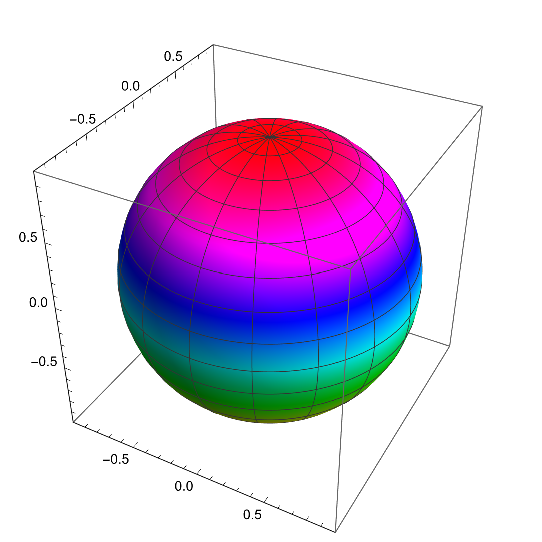
\includegraphics[ width = 1.5in ]{\pLocalGraphics bw/scission-000.pdf} &
	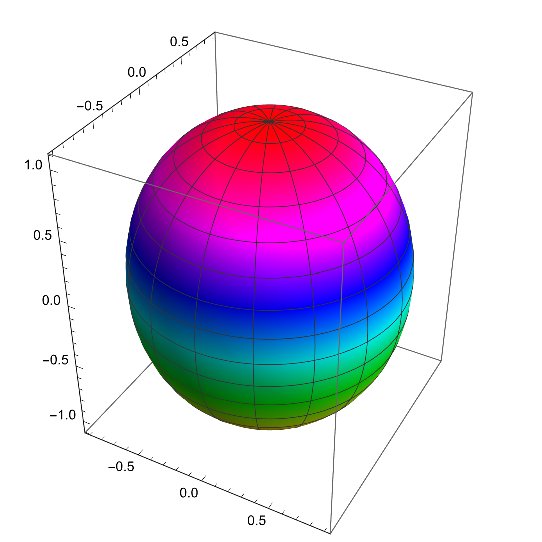
\includegraphics[ width = 1.5in ]{\pLocalGraphics bw/scission-001.pdf} &
	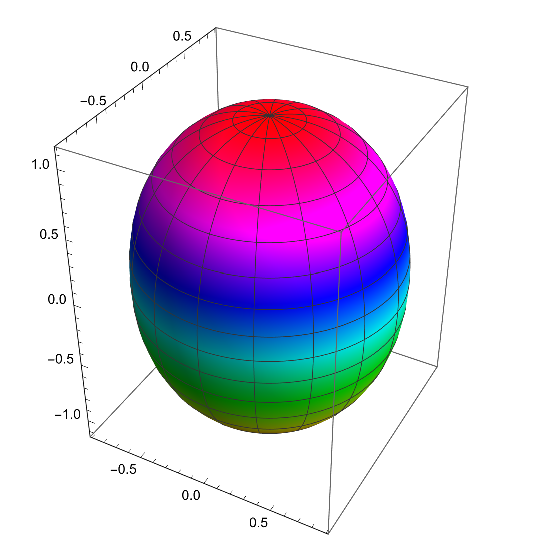
\includegraphics[ width = 1.5in ]{\pLocalGraphics bw/scission-002} \\
\end{tabular}
\end{center}
%\label{default}
\end{table}
\end{frame}

\begin{frame}\frametitle{Early Scission Sequence}
\begin{table}[htp]
%\caption{default}
\begin{center}
\begin{tabular}{cccc}
		%
	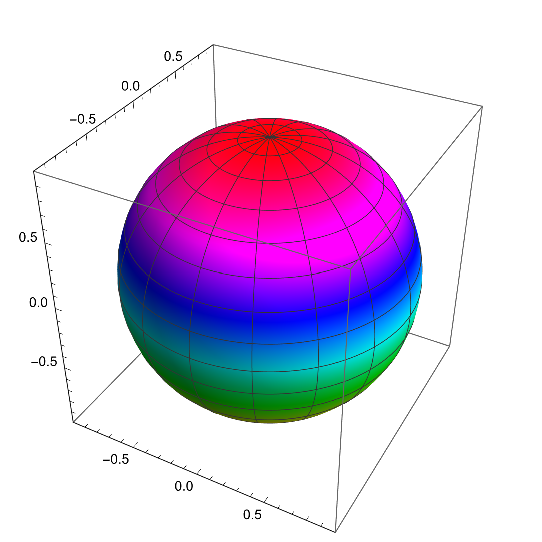
\includegraphics[ width = 1.0in ]{\pLocalGraphics bw/scission-000} &
	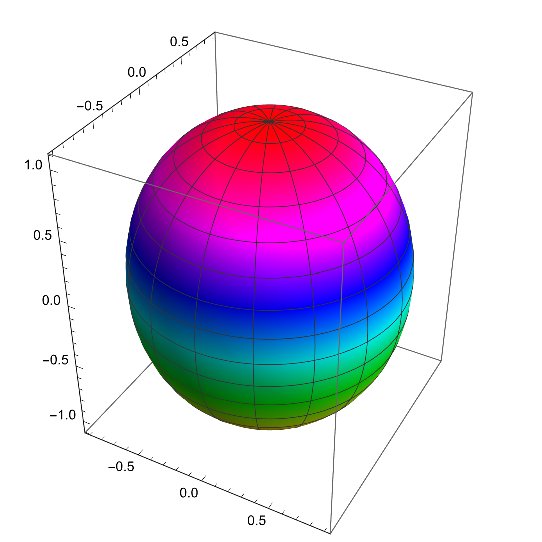
\includegraphics[ width = 1.0in ]{\pLocalGraphics bw/scission-001} &
	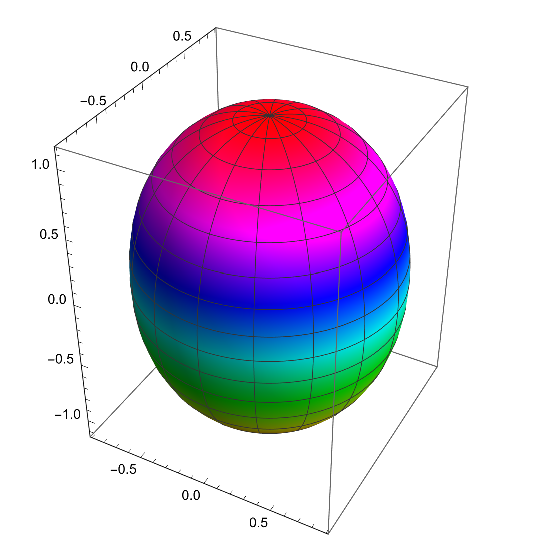
\includegraphics[ width = 1.0in ]{\pLocalGraphics bw/scission-002} &
	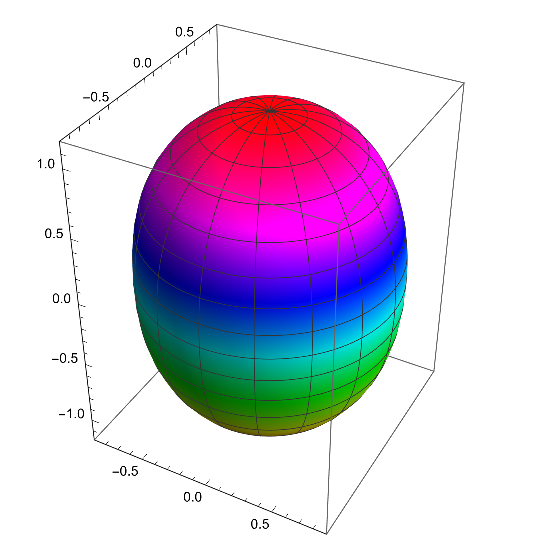
\includegraphics[ width = 1.0in ]{\pLocalGraphics bw/scission-003} \\
		%
	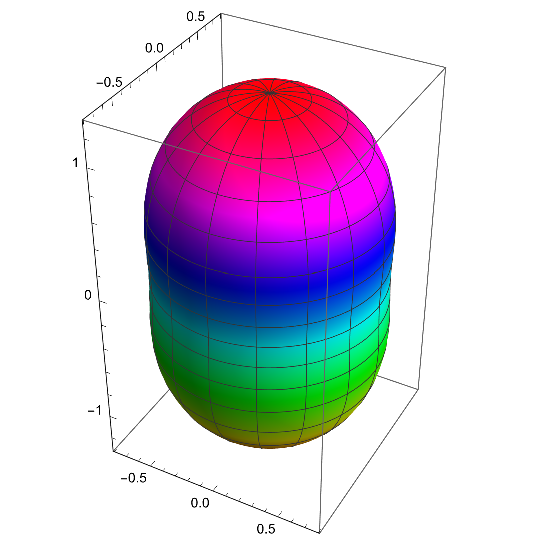
\includegraphics[ width = 1.0in ]{\pLocalGraphics bw/scission-010} &
	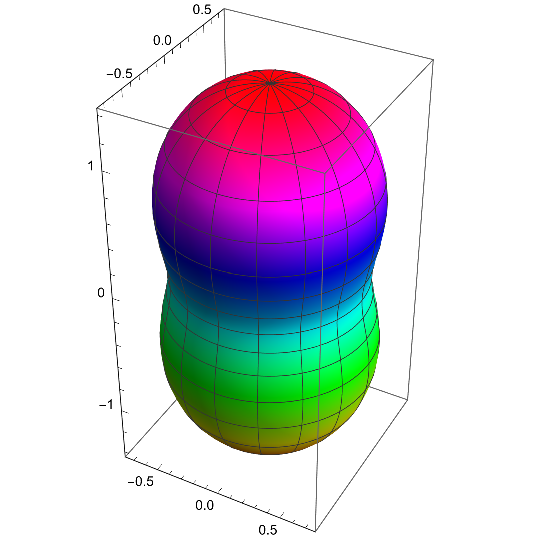
\includegraphics[ width = 1.0in ]{\pLocalGraphics bw/scission-020} &
	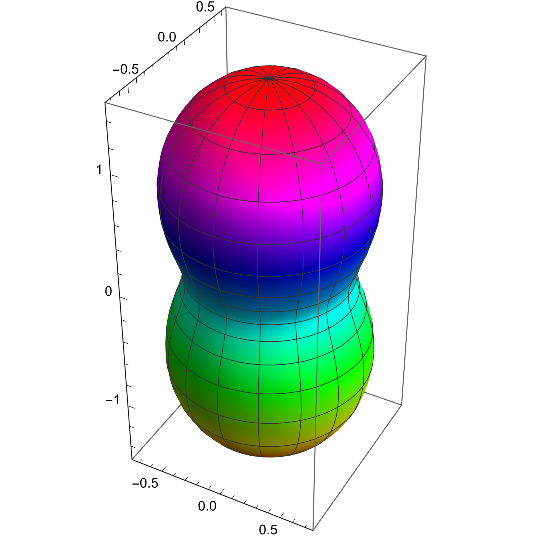
\includegraphics[ width = 1.0in ]{\pLocalGraphics bw/scission-030} &
	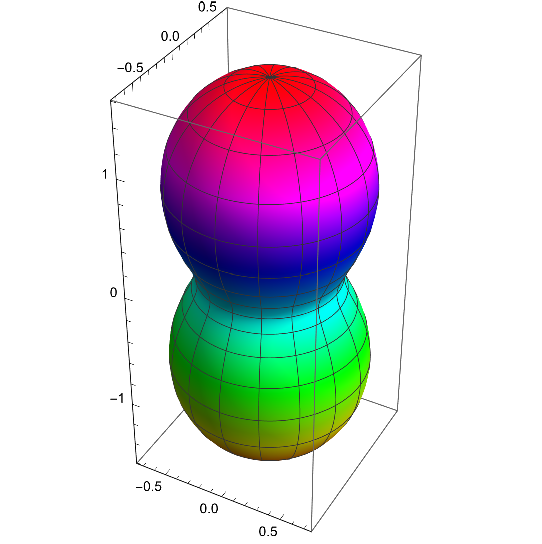
\includegraphics[ width = 1.0in ]{\pLocalGraphics bw/scission-040} \\
		%
\end{tabular}
\end{center}
%\label{default}
\end{table}
\end{frame}

\begin{frame}\frametitle{Late Scission Sequence}
\begin{table}[htp]
%\caption{default}
\begin{center}
\begin{tabular}{cccc}
		%
	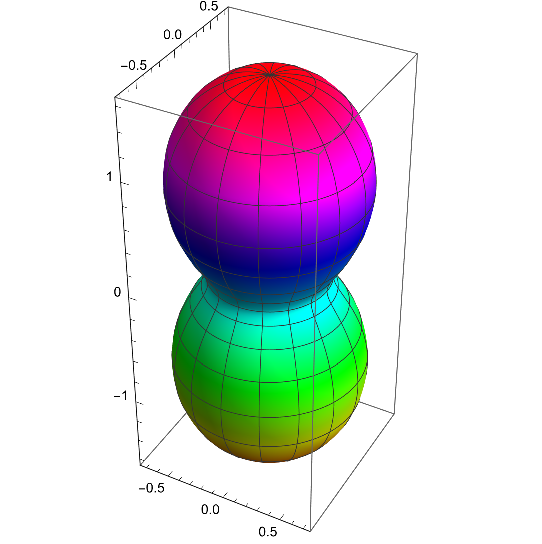
\includegraphics[ width = 1.0in ]{\pLocalGraphics bw/scission-050} &
	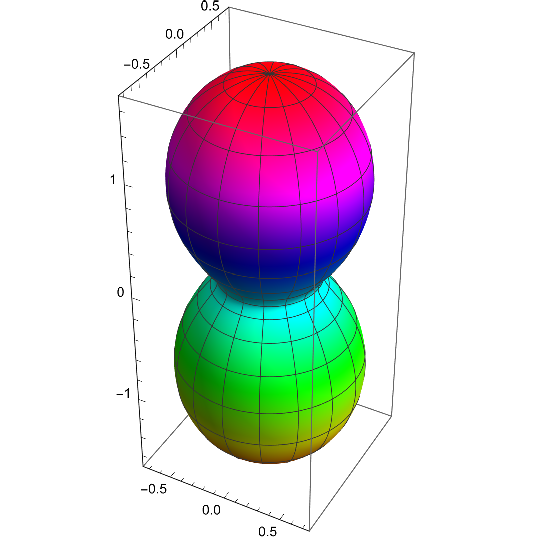
\includegraphics[ width = 1.0in ]{\pLocalGraphics bw/scission-060} &
	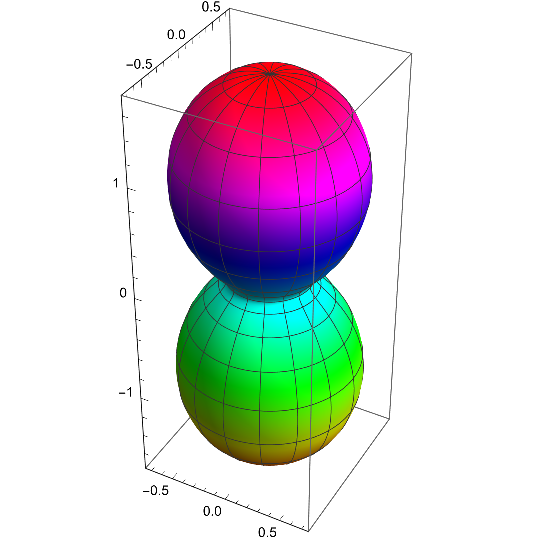
\includegraphics[ width = 1.0in ]{\pLocalGraphics bw/scission-070} &
	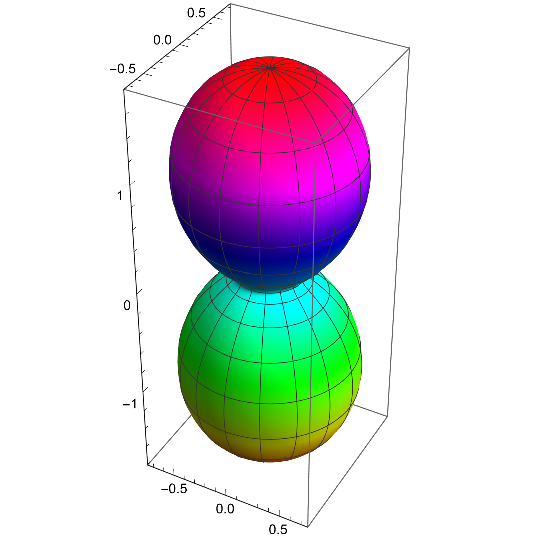
\includegraphics[ width = 1.0in ]{\pLocalGraphics bw/scission-080} \\
		%
	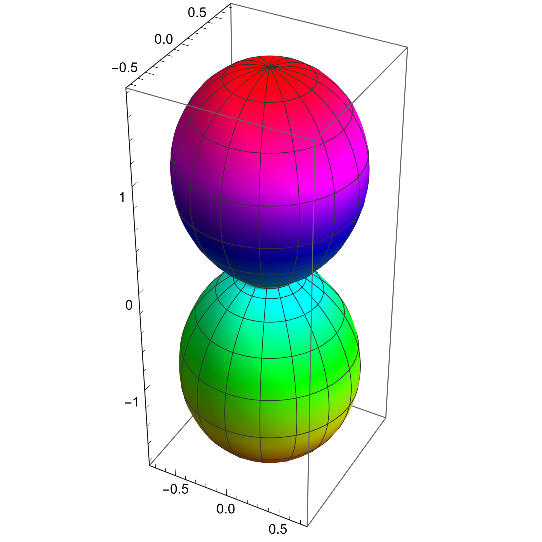
\includegraphics[ width = 1.0in ]{\pLocalGraphics bw/scission-090} &
	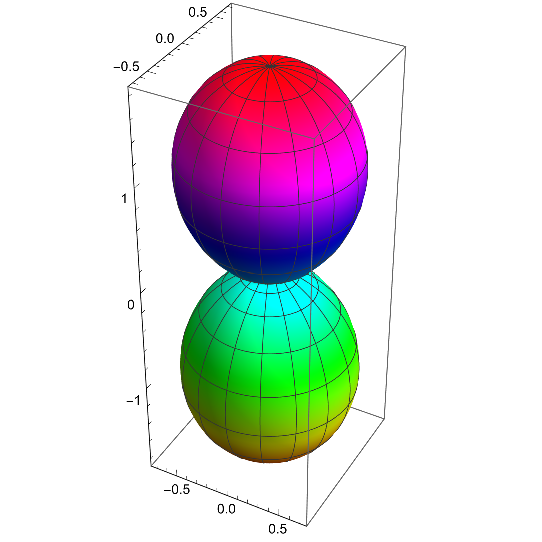
\includegraphics[ width = 1.0in ]{\pLocalGraphics bw/scission-100} &
	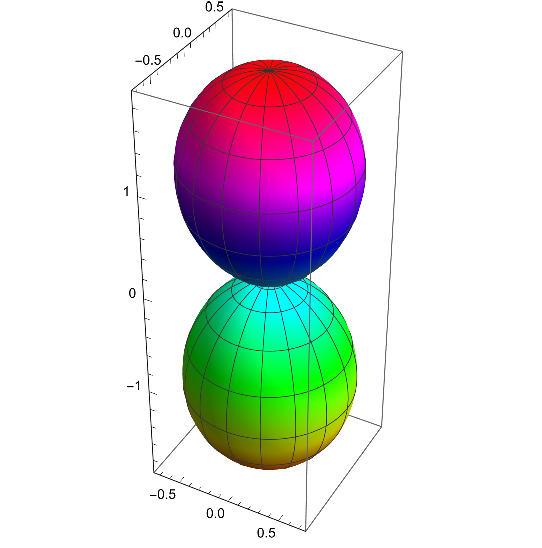
\includegraphics[ width = 1.0in ]{\pLocalGraphics bw/scission-120} &
	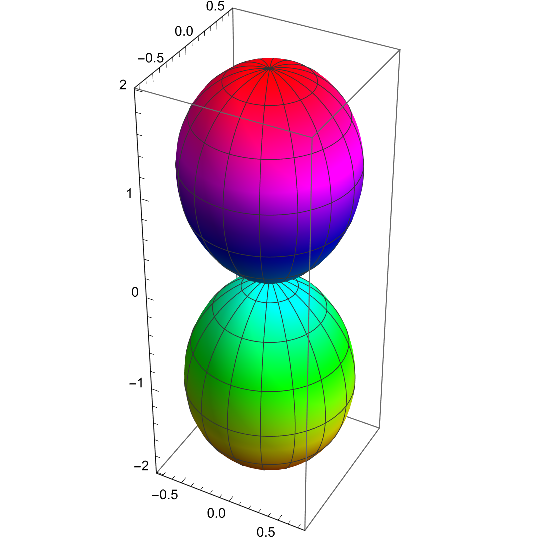
\includegraphics[ width = 1.0in ]{\pLocalGraphics bw/scission-140} \\
		%
\end{tabular}
\end{center}
%\label{default}
\end{table}
\end{frame}

\begin{frame}\frametitle{Scission Sequence Outlines}
\begin{table}[htp]
%\caption{default}
\begin{center}
\begin{tabular}{cccc}
		%
	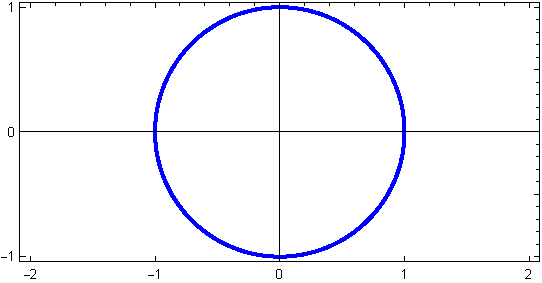
\includegraphics[ width = 1.0in ]{\pLocalGraphics bw/peanut-000.pdf} &
	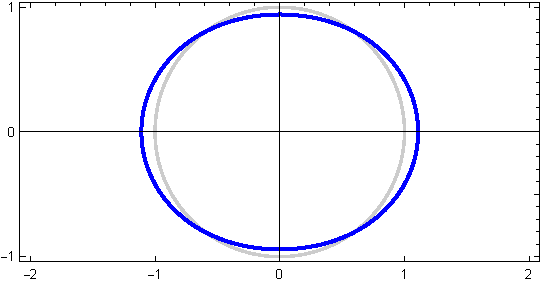
\includegraphics[ width = 1.0in ]{\pLocalGraphics bw/peanut-001.pdf} &
	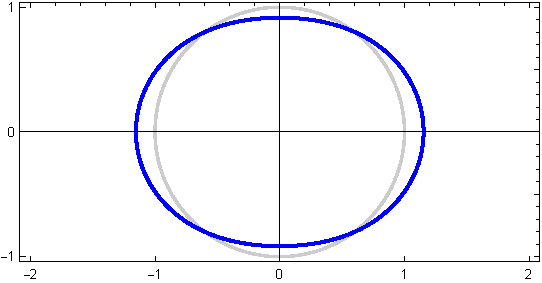
\includegraphics[ width = 1.0in ]{\pLocalGraphics bw/peanut-002.pdf} &
	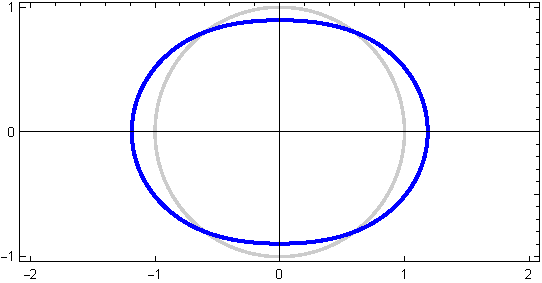
\includegraphics[ width = 1.0in ]{\pLocalGraphics bw/peanut-003.pdf} \\[10pt]
		%
	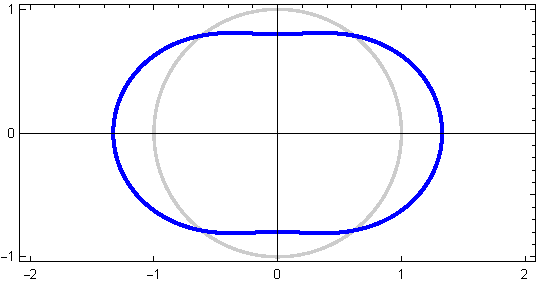
\includegraphics[ width = 1.0in ]{\pLocalGraphics bw/peanut-010.pdf} &
	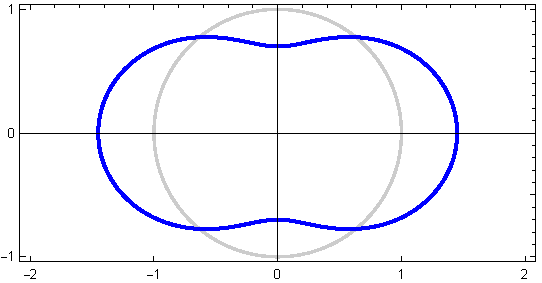
\includegraphics[ width = 1.0in ]{\pLocalGraphics bw/peanut-020.pdf} &
	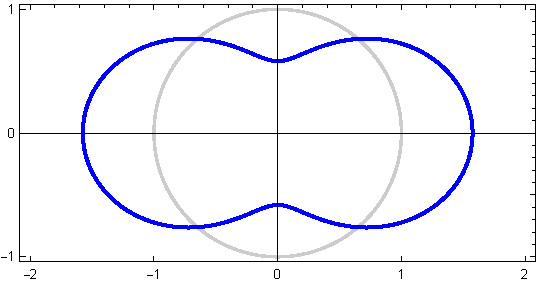
\includegraphics[ width = 1.0in ]{\pLocalGraphics bw/peanut-035.pdf} &
	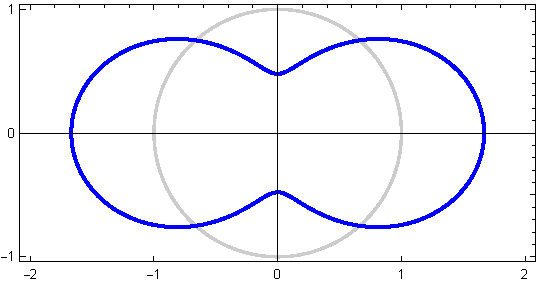
\includegraphics[ width = 1.0in ]{\pLocalGraphics bw/peanut-050.pdf} \\[10pt]
		%
	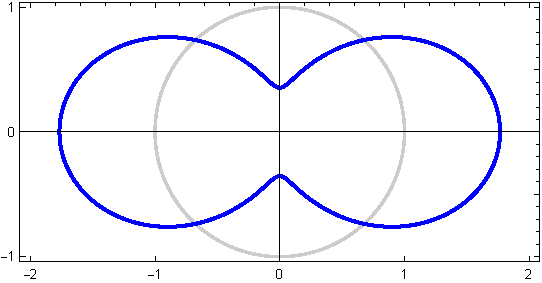
\includegraphics[ width = 1.0in ]{\pLocalGraphics bw/peanut-070.pdf} &
	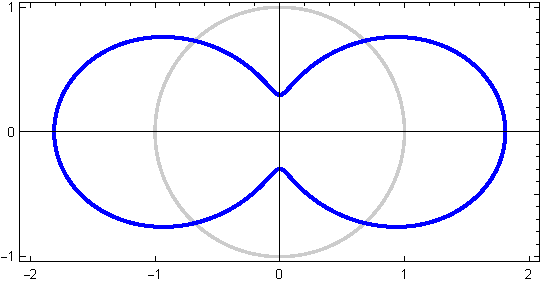
\includegraphics[ width = 1.0in ]{\pLocalGraphics bw/peanut-080.pdf} &
	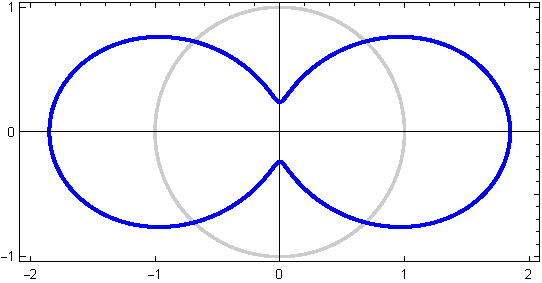
\includegraphics[ width = 1.0in ]{\pLocalGraphics bw/peanut-090.pdf} &
	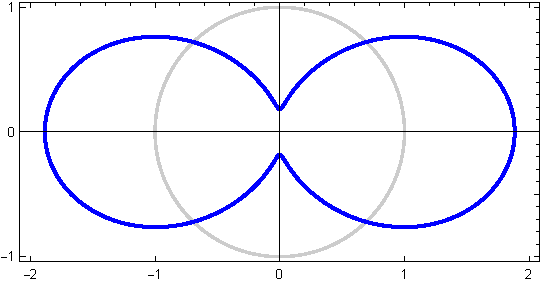
\includegraphics[ width = 1.0in ]{\pLocalGraphics bw/peanut-100.pdf} \\
		%
\end{tabular}
\end{center}
%\label{default}
\end{table}
\end{frame}

\begin{frame}\frametitle{Separation Sequence}
\center
	\href{http://aip.scitation.org/doi/abs/10.1063/1.4725468}{
	\begin{overpic}[ scale = 1.0 ]
	{\pLocalGraphics binocular-plot}
		%\put(0,0){Text}
	\end{overpic}}
\end{frame}


\begin{frame}\frametitle{Bohr--Wheeler Deformation Sequence}
\center
	\href{https://link.aps.org/pdf/10.1103/PhysRev.56.426}{
	\begin{overpic}[ scale = 0.95 ]
	{\pLocalGraphics bw/path-deformation.pdf}
		\put(50,-3){$\azero$}
		\put(-7,32){$\atwo$}
		\put(100,-5){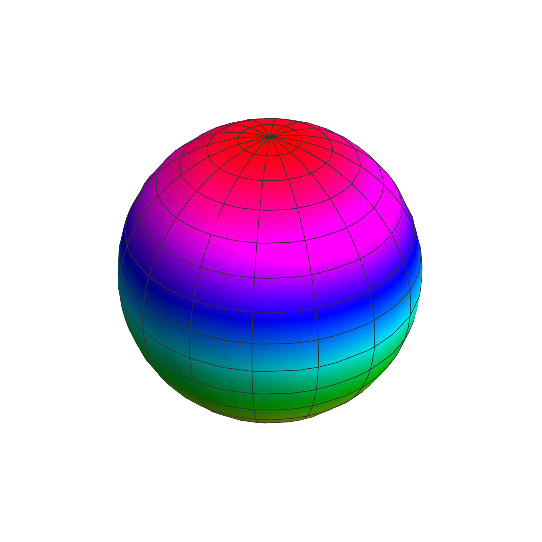
\includegraphics[ scale = 0.2 ]{\pLocalGraphics bw/shape-sphere.pdf}}
		\put(-15,50){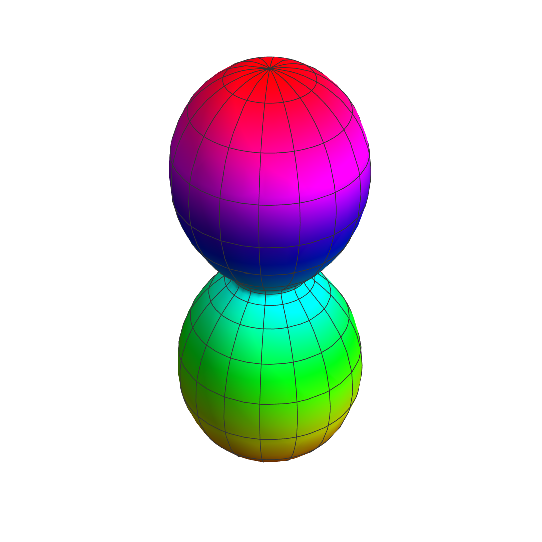
\includegraphics[ scale = 0.2 ]{\pLocalGraphics bw/shape-dumbells.pdf}}
	\end{overpic}}
\end{frame}

\begin{frame}\frametitle{Bohr--Wheeler Error in Volume}
\center
	\href{https://link.aps.org/pdf/10.1103/PhysRev.56.426}{
	\begin{overpic}[ scale = 0.95 ]
	{\pLocalGraphics bw/volume-error.pdf}
		\put(50,-2){step}
		\put(-6,19){\rotatebox{90}{Volume error}}
		\put(100,-5){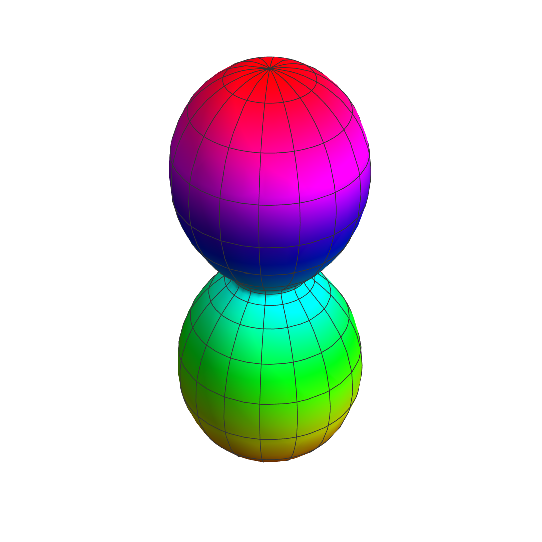
\includegraphics[ scale = 0.2 ]{\pLocalGraphics bw/shape-dumbells.pdf}}
		\put(-16,50){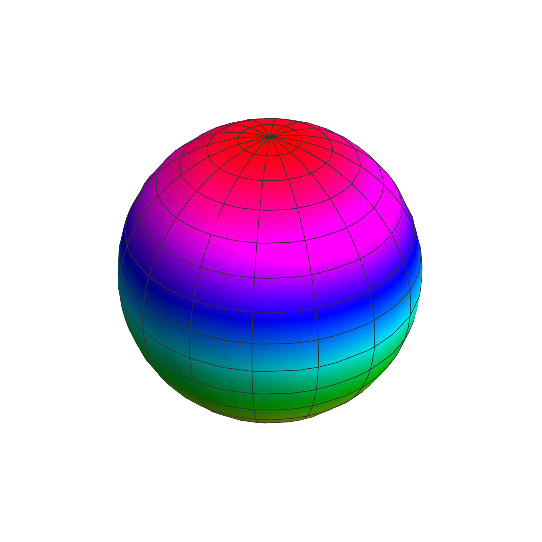
\includegraphics[ scale = 0.2 ]{\pLocalGraphics bw/shape-sphere.pdf}}
	\end{overpic}}
\end{frame}

%\begin{frame}
%	\frametitle{References for Bohr-Wheeler Fission Limit}
%	\begin{enumerate}
%		\item \href{https://link.aps.org/pdf/10.1103/PhysRev.56.426}{The Mechanism of Nuclear Fission}
%		\item \href{https://link.springer.com/book/10.1007/978-3-642-14709-8}{The Physics Of The Manhattan Project, \S 6.5}
%		\item \href{https://iopscience.iop.org/article/10.1088/0143-0807/30/4/009}{The Bohr–Wheeler spontaneous fission limit: an undergraduate-level derivation}
%		\item \href{https://link.aps.org/doi/10.1103/PhysRev.72.914}{Calculations in the Liquid-Drop Model of Fission}
%	\end{enumerate}
%\end{frame}

\endinput  %  ==  ==  ==  ==  ==  ==  ==  ==  ==
